% !TEX encoding = UTF-8 Unicode 
% !TEX root = praca.tex
\graphicspath{{chapters/chapter1/imgs/}}

\chapter{Narracja w grach}\label{chapter:ch1}

Niniejszy rozdział ma na celu dokonanie przeglądu gier komputerowych na przestrzeni lat, ze
szczególnym naciskiem na ewolucję sposobów oraz form narracji przedstawianych w tych grach.
Wyszczególnione zostaną również naistotniejsze struktury i rodzaje narracji, które są współcześnie
wykorzystywane. Dodatkowo, nastąpi krótki przegląd najpopularniejszych technik prezentacji narracji.
Na koniec nakreślone zostaną systemy dialogowe wykorzystywane przez gry komputerowe.

\section{Historia narracji w grach komputerowych}\label{section:ch1_1}

Aby zrozumieć istotę narracji w grach komputerowych, należy przede wszystkim określić
co może kryć się pod tym pojęciem. Pozwoli to dokonać przeglądu wybranych tytułów
i wyciągnąć z tego przeglądu wnioski. Żeby udowodnić rozwój w sposobie prezentowania narracji
na przestrzeni lat, prześledzone zostały części jednej z serii gier --- \textit{"Final Fantasy"} ---
wydawanej od roku 1987.

\subsection{Definicja narracji}\label{subsection:ch1_1_1}

Pojęcie narracji i samo jej występowanie w grach komputerowych jest kwestią sporną
w literaturze od lat. Barry Ip, w swojej pracy \cite{narrative_structures}, dokonuje wyróżnienia trzech słów ściśle
powiązanych ze sobą: \textit{historia}, \textit{fabuła} oraz \textit{narracja}. Na potrzeby jego
badań historia zdefiniowana została następująco:

\begin{quotation}
	\ldots \textit{sekwencja zdarzeń obejmujących byty.} \cite{narrative_structures}
\end{quotation}

Związana z historią jest również fabuła, która została określona przez Arystotelesa jako:

\begin{quotation}
	\ldots \textit{organizacja zdarzeń.} \cite{narrative_structures}
\end{quotation}

Sama narracja, ściśle powiązana z dwoma poprzednimi terminami, wyrażona została w sposób
następujący:

\begin{quotation}
	\ldots \textit{reprezentacja zdarzenia lub serii zdarzeń.} \cite{narrative_structures}
\end{quotation}

W ramach tej pracy, można przyjąć wszystkie te pojęcia jako istotne i na tyle bliskie
siebie, że mogą być wykorzystywane zamiennie.

Jakub Majewski sugeruje, że debatowanie nad istnieniem narracji jest odpowiednie dla niektórych
gier, a dla niektórych nie \cite{theorising_narrative}. Rozdzielenie bowiem tych form
przekazu, które można zaliczyć do treści fabularnej, nie jest takie oczywiste. Przytoczyć można
przykład \textit{Space Invaders} (1977) --- gra nie przytacza żadnego opisu w formie tekstowej,
skupiając się wyłącznie na rozgrywce. Na podstawie samego tytułu można jednak
przypuścić, że dokonuje się pewnego rodzaju inwazja, a stoją za nią przybysze z kosmosu \cite{theorising_narrative}.

Ten przykład pokazuje, że granica między grami posiadającymi narrację a tymi, w których jest ona nieobecna,
może być płynna. Nawet gry pozbawione bezpośrednich opisów fabularnych mogą zawierać pewne nawiązania narracyjne,
które wynikają z innych elementów, takich jak tytuł czy grafika. W związku z tym, podział na gry z narracją i bez
narracji może być problematyczny, ponieważ elementy narracyjne mogą przejawiać się w różnych formach i stopniach
w różnych grach. Jako że nie jest to główny problem poruszany w niniejszej pracy to wszystko co może być elementem
narracyjnym, jest za taki uznawany.

Do budowania narracji w grach wykorzystane mogą być wzorce znane z literatury. Przykładem takiego wzorca jest
\textit{"Podróż bohatera"}\cite{narrative_structures}, który opisuje 12 kluczowych etapów, odgrywających
istotną rolę w budowie angażujących historii (Tabela \ref{tab1:ch1_1_1}). Blisko powiązana z \textit{"Podróżą bohatera"}
jest znana struktura trzech aktów opisana przez Arystotelesa, która zakłada podział utworu na
początek, środek i koniec\cite{narrative_structures}. Jest to bardzo elastyczna a zarazem bardzo ogólna metoda
podziału. Zasadniczo w każdym utworze dałoby się bowiem w pewien sposób wyodrębnić te akty.

Struktury te pozwalają projektantom fabuły konstruować spójny świat fikcji --- niezależnie od formy w
jakiej zostanie zaprezentowana odbiorcom. Takowa może być adaptowana zarówno do powieści, jak i do materiału
filmowego czy też gier komputerowych.

\begin{table}[h!]
	\caption{Dwanaście etapów wzorca narracyjnego "Podróży bohatera" \cite{narrative_structures}}
	\label{tab1:ch1_1_1}
	\begin{center}
		\begin{tabular}{p{1.5in} p{4in}}
			\hline
			Etap                                & Opis                                                                                                                                                                                                                                                                                                                            \\
			\hline
			1. Zwyczajny świat                  & Gracz po raz pierwszy spotyka bohatera i zapoznaje się z jego pochodzeniem, zazwyczaj za pośrednictwem historii drugoplanowej                                                                                                                                                                                                   \\
			2. Wezwanie do przygody             & Wskazówka, że bohater opuści zwykły świat, by rozpocząć nową przygodę. Ten etap działa jak katalizator, który uruchamia główny wątek fabularny                                                                                                                                                                                  \\
			3. Odrzucenie wezwania              & W tradycyjnej strukturze monomitu bohater odrzuca początkową propozycję opuszczenia zwykłego świata i rozpoczęcia misji, zwykle w chwili wątpliwości lub niepewności                                                                                                                                                            \\
			4. Spotkanie z mentorem             & Gdy bohater decyduje się na podjęcie zadania, mentor dostarcza mu informacji potrzebnych do podjęcia decyzji. Mentorem może być wszystko, co dostarcza informacji - brodaty starzec, robot, biblioteka, doświadczenia z przeszłości i tak dalej                                                                                 \\
			5. Przekroczenie pierwszego progu   & Bohater przechodzi z bezpiecznego zwykłego świata do nowego, niebezpiecznego i nieznanego świata poszukiwań                                                                                                                                                                                                                     \\
			6. Testy, sprzymierzeńcy i wrogowie & Faza ta jest zwykle największą częścią fabuły gry, ponieważ gracz poznaje wszystkie główne postacie                                                                                                                                                                                                                             \\
			7. Podejście do najgłębszej jaskini & Jest to miejsce, w którym bohater znajduje nagrodę, której szuka - taką jak zdobycie niezbędnej umiejętności, broni lub opanowanie wszystkiego, co napotkał do tej pory. Zazwyczaj ma to miejsce pod koniec gry. Głównym celem tej części historii jest przygotowanie bohatera do ostatecznej bitwy                             \\
			8. Próba                            & To tutaj bohater staje do ostatecznej walki ze swoim nemezis lub "ostatecznym bossem". Nemezis może pojawić się jako byt fizyczny (osoba lub przedmiot) lub niefizyczny (czas, intensywność lub trudność)                                                                                                                       \\
			9. Nagroda                          & Wiele gier kończy się w tym momencie, gdy wróg zostaje pokonany, a nagrodą jest zazwyczaj końcowa cut-scenka opisująca, co dzieje się z bohaterem po jego triumfie                                                                                                                                                              \\
			10. Droga powrotna                  & Niektóre gry pozwolą graczowi powrócić do zwykłego świata po otrzymaniu nagrody, ale może nie być możliwe, aby bohater z powodzeniem zintegrował się ze starym światem                                                                                                                                                          \\
			11. Wksrzeszenie                    & Ta część historii odpowiada na wszelkie pytania bez odpowiedzi, takie jak konsekwencje misji, potencjalne konflikty, które mogą pojawić się w przyszłych sequelach, lub wszelkie testy, którym bohater musi stawić czoła przed końcem. Może mieć również formę ostatecznego zwrotu akcji, jako coś nieoczekiwanego przez widzów \\
			12. Powrót z nagrodą                & Jest to ostatni etap historii, w którym bohater w końcu powraca do zwykłego świata i widzi korzyści płynące z jej nagrody. Bohater może porównać swoje życie przed i po wyprawie, aby zobaczyć, jak wszystko się zmieniło                                                                                                       \\
			\hline
		\end{tabular}
	\end{center}
\end{table}

\newpage

\subsection{Przedstawienie narracji w grach na przestrzeni lat}\label{subsection:ch1_1_2}

Kamienie milowe w początkach branży gier wideo to: Spacewar (Rys \ref{fig:ch1_1_2_spacewar}) - pierwsza interaktywna gra z
1962 roku, Odyseja Magnavoksa - pierwszy domowy system gier podłączany do telewizora (1972), a
także Pong (Rys \ref{fig:ch1_1_2_pong}) od Atari (1972) i przenośne gry LED Mattela (1977)\cite{the_evolution_of_video_games}.

TODO screeny ponga i spacewar + krótki opis

\begin{figure}[h]
	\caption{Spacewar (1962)}
	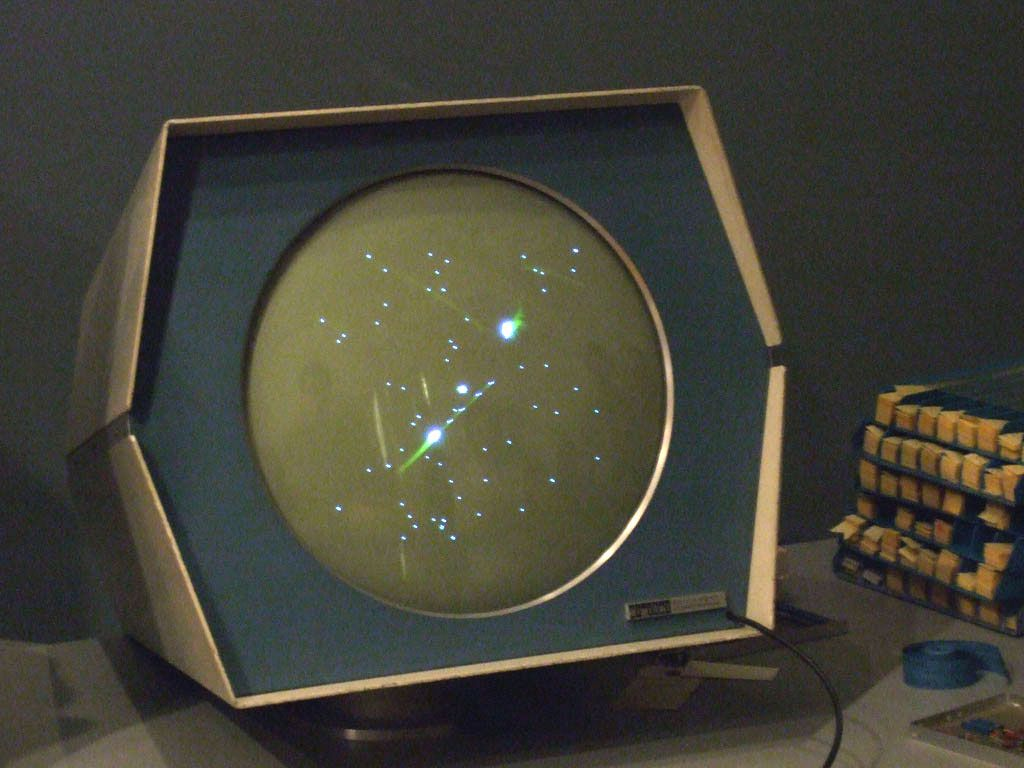
\includegraphics[width=0.5\textwidth]{ch1_1_2_spacewar.jpg}
	\centering
	\label{fig:ch1_1_2_spacewar}
\end{figure}

\begin{figure}[h]
	\caption{Pong (1972)}
	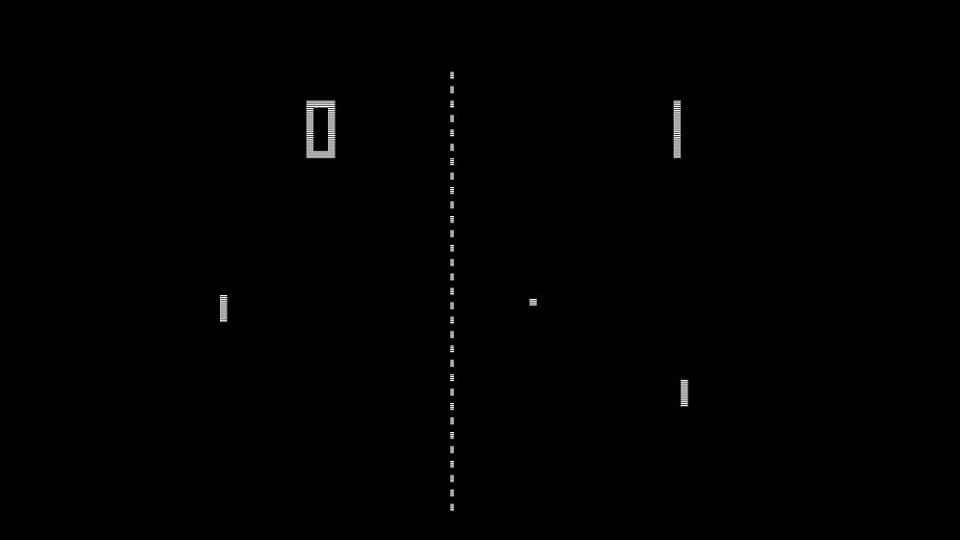
\includegraphics[width=0.5\textwidth]{ch_1_1_2_pong.jpg}
	\centering
	\label{fig:ch1_1_2_pong}
\end{figure}

Lata 70. przyniosły rozwój firm jak Atari, Nintendo i Sega oraz pierwsze hity salonów
gier np. Pacman (1980), który sprzedał 300 000 sztuk na całym świecie\cite{the_evolution_of_video_games}.

TODO Atari Breakout + Space Invaders

W latach 80. nastąpił boom konsol domowych - Nintendo NES, Sega Master System, Atari 7800 (1986)\cite{the_evolution_of_video_games}.

TODO Super Mario Bros + The Legend of Zelda (z full walktrough wywnioskować)

Dekadę później gry komputerowe PC zyskały popularność dzięki tytułom jak Doom, a na rynku
pojawiły się PlayStation i Nintendo 64. Koniec XX wieku to także rozwój przenośnych gier na
fali sukcesu serii Pokemon.

TODO Crash Bandicoot / Spyro + Half Life

Nowe millennium przyniosło dalszy rozwój branży do rozmiarów dzisiejszej potęgi, poprzez stale
pojawiające się innowacje sprzętowe i nowe przełomowe tytuły na różne platformy.

TODO wybrać 2-3 tytuły (Life is Strange + ??? + ???) i krótki opis możliwości narracyjnych

\subsection{Prześledzenie rozwoju narracji na przykładzie serii Final Fantasy}\label{subsection:ch1_1_3}

goiemgoe

\section{Rodzaje narracji w grach komputerowych}\label{section:ch1_2}

efe

\subsection{Struktury narracji}\label{subsection:ch1_2_1}

fefef

\subsection{Rodzaje narracji}\label{subsection:ch1_2_2}

fefef

\subsection{Techniki przedstawienia narracji}\label{subsection:ch1_2_3}

ioegemo

\section{Systemy dialogowe w grach komputerowych}\label{section:ch1_3}

fefef

\subsection{Popularne systemy dialogowe}\label{subsection:ch1_3_1}

fefef

\subsection{Interaktywna fikcja - system poleceń}\label{subsection:ch1_3_2}

ortatraoitrmoi